\RequirePackage{luatex85}
\documentclass[tikz]{standalone}

\usepackage{tikz-feynman}

\begin{document}
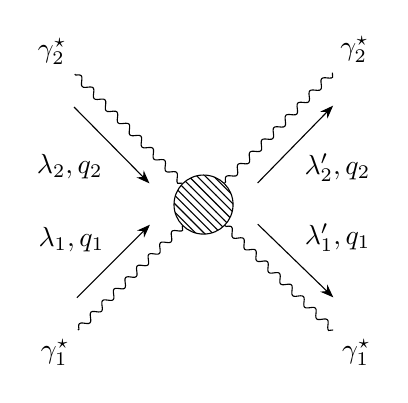
\begin{tikzpicture}

    \begin{feynman}
        \diagram [horizontal=in1 to out1,medium] {
            in1 [particle=\(\gamma_{1}^\star\)] -- [photon, momentum={\(\lambda_1, q_1\)}] mess [blob] -- [photon, momentum={\(\lambda_1^\prime, q_1\)}] out1 [particle=\(\gamma_1^\star\)],
            in2 [particle=\(\gamma_{2}^\star\)] -- [photon, momentum'={\(\lambda_2, q_2\)}] mess -- [photon, momentum'={\(\lambda_2^\prime, q_2\)}] out2 [particle=\(\gamma_2^\star\)],
            in1 -- [plain, opacity=0] in2,
            out1 -- [plain, opacity=0] out2,
            in1 -- [plain, opacity=0] out1,
            in2 -- [plain, opacity=0] out2,
        };
    \end{feynman}
\end{tikzpicture}
\end{document}
